\chapter{Methodologies}
\label{cha:methodologies}



Throughout this chapter, the methodologies used to approach the research
objectives are explained. It describes the feature engineering and extraction
methods, the way explainable AI methods are used, model training and
optimization approaches, clustering and dimensionality reduction techniques and
statistical hypotheses testing methods.
%---------------------------------------------------------------------------

\section{Feature Engineering}
\label{sec:featureengineering}

Feature engineering is a vital step in the research process, as it involves
transforming raw data acquired using the data collection script into meaningful
representations that can be analyzed or used for predictive modeling. In this
section the methodologies used to get acoustic features from the mp3 files and
lyrical features from the lyrics are described. These features are designed to
capture key characteristics of the songs, enabling deeper insights into their
patterns and relationships.


\subsection{Acoustic Features}
\label{sec:acousticfeatures}

These features provide a numeric representation of the acoustic properties of
each song and were extracted directly from the audio files in MP3 format. They
describe different aspects of audio signal and provide information about the
rhythm, timbre, harmony and other acoustic properties. The extraction was done
using \textit{Librosa} and was automated and parallelized to make it suitable
for processing large amounts of data. \cite{librosa}


\subsubsection*{MFCC - Mel Frequency Cepstral Coefficients}
MFCCs are used to analyze the short-term power spectrum of a song on a
mel-scale. They're also used for timbre analysis, and they capture the tonal
quality of the audio, which helps differentiate between different instruments
and vocal characteristics. After some trial and error and taking into
consideration the resources available for the extraction of those features and
model training, thirteen MFCC coefficients were calculated for each track.




\subsubsection*{Chroma}
Chroma vectors represent the intensity of each pitch class (e.g., C, C#, D,
etc.) in the audio. These features provide a harmonic representation of the
song and are useful for analyzing chord progressions and harmonic structures.
For each track 12 Chroma features were extracted.

\subsubsection*{Spectral Contrast}
Spectral contrast measures the difference in amplitude between peaks and
valleys in the spectrum. It provides insights into the harmonic and timbral
content of a song, particularly useful for distinguishing between smooth and
complex textures. Seven features were extracted for every song.

\subsubsection*{Other Features}
Two additional features were extracted:
\begin{itemize}
  \item \textbf{Tempo} - speed of the song, measured in
    \textit{Beats Per Minute (BPM)};
  \item \textbf{Zero Crossing Rate (ZCR)} - measures the rate at which the audio
    signal changes sign. Commonly used as a measure of noisiness or
    percussive nature of signal.
\end{itemize}

%---------------------------------------------------------------------------

\subsection{Lyrical Features}
\label{sec:lyricalfeatures}

Lyrical features  were extracted from the lyrics fetched during the data
collection process. They aim to provide a linguistic and semantic
representation of the track, capturing their complexity, sentiment and
stylistic  attributes. In the cleaning and extraction  process various NLP
libraries like \textit{NLTK}, \textit{spaCy} and \textit{TextBlob} were used,
alongside with custom ad-hoc algorithms. Before extraction the lyrics  had to
be carefully cleaned, removing unnecessary characters and stopwords, performing
stemming etc.\cite{nltk,spacy,textblob} 

Similarily to acoustic features the implementation allowed for simple and
intuitive usage  with parallelization of the computation process for increased
performance. 

The features extracted can be grouped as follows:

\subsubsection*{Basic Linguistic Metrics}
\begin{itemize}
  \item \textbf{Unique Word Count} - measures number of unique words in the
    lyrics, indicating diversity;
  \item \textbf{Type-Token Ratio} - measures of lexical richness: ratio of
    unique words to total words;
  \item \textbf{Word Count} - total  number of words;
  \item \textbf{Noun and Verb Ratios} - proportions of nous and verbs relative
    to the total word count.
\end{itemize}


\subsubsection*{Sentiment and Emotional Tone}
\begin{itemize}
  \item \textbf{Sentiment Polarity} - a measure of overall sentiment (positive
    vs. negative) of the text;
  \item \textbf{Sentiment Subjectivity} - represents the degree of subjectivity
    in the lyrics;
  \item \textbf{VADER Compound} - a sentiment score obtained using VADER;
  \item \textbf{Sentiment Variability} - standard deviation of sentiment on
    subsets of lyrics. This metric aims to capture changes in sentiment
    throughout the song.
\end{itemize}


\subsubsection*{Stylistic Features}
\begin{itemize}
  \item \textbf{Repetition Count} - the frequency of repeated words;
  \item \textbf{Rhyme Density} - a measure of how often rhymes occur in the
    text;
  \item \textbf{Linguistic Uniqueness} - ratio of rarely used words to all the
    words in the song.
\end{itemize}


\subsubsection*{Semantic and Complexity Features}
\begin{itemize}
  \item \textbf{Semantic Depth} - represents the richness and variety of
    meaning of the lyrics;
  \item \textbf{Syntactic Complexity} - captures the sophistication of
    sentence structures;
  \item \textbf{Lexical Richness} - quantifies the variety and richness of the
    vocabulary.
\end{itemize}



\subsubsection*{Readability and Accessibility}
\begin{itemize}
  \item \textbf{Flesch Reading Ease} - indicates how easy the lyrics are to
    read;
  \item \textbf{Gunning Fog} - a metric that estimates the  years of education
    required to understand the text;
  \item \textbf{Dale Chall} - a metric that accounts for familiar and
    unfamiliar words in the text.
\end{itemize}


\subsubsection*{Contextual Information}
  In process of feature extraction the \textbf{language} of lyrics was also
  identified using \textit{langdetect} library. Langdetect uses a
  classification model to predict the language of a text based on n-grams from
  it. The identified language was also used cleaning process, to remove songs
  that weren't in English.

\subsubsection*{TF-IDF (Term Frequency - Inverse Document Frequency)}

TF-IDF is a measure that can quantifies the relevance of tokens in a
document in a collection of documents. It's used to highlight words that are unique or
meaningful while giving less importance to very common words like 'the' or
'and'.\cite{tfidf}

It can be broken down into two parts:


\begin{itemize}
  \item \textbf{TF - Term Frequency} - Measures the frequency of a term within
    a document:
  \[
  TF(w, d) = \frac{f_{w, d}}{N_d}
  \]
  where:
  \begin{itemize}
    \item \( f_{w, d} \): The number of times the word \( w \) appears in the
      document \( d \);
    \item \( N_d \): The total number of words in the document \( d \).
  \end{itemize}

  \item \textbf{IDF - Inverse Document Frequency} - Measures the rarity of a
    term across a collection of documents:
  \[
  IDF(w) = \log{\frac{N}{1 + n_w}}
  \]
  where:
  \begin{itemize}
    \item \( N \): The total number of documents in the corpus;
    \item \( n_w \): The number of documents containing the word \( w \).
  \end{itemize}
\end{itemize}


The final TF-IDF value is calculated by multiplying the Term Frequency (TF) and
the Inverse Document Frequency (IDF) for a word \( w \):  
\[  
TF\text{-}IDF(w, d) = TF(w, d) \cdot IDF(w)  
\]  

Terms that occur frequently in a specific document (high TF) and rarely appear
in other documents (high IDF) receive a higher score.

\subsubsection*{Word2Vec}

Word2Vec is a neural network-based technique in NLP for creating dense vector
representations of words. These vectors capture information about the meaning
of words based on the surrounding words. Unlike bag-of-words or TF-IDF methods,
Word2Vec generates embeddings that preserve the contextual meaning of words
based on their usage within the corpus.\cite{w2v}

Two primary approaches are used in Word2Vec: 
\begin{itemize} 
  \item \textbf{Continuous Bag of Words}: Predicts a target word based
    on its surrounding context words;
  \item \textbf{Skip-Gram}: Predicts context words given a target word.
\end{itemize}

In this study, Word2Vec was used to create vector representations of song
lyrics. These embeddings  were used similarily to TF-IDF, as input features
to predictive models and when comparing lyrical similarities between genres.



\subsubsection*{Empath}
Empath is a semantic analysis tool designed for extracting
semantic, thematic and emotional features from text by analyzing words based on
predefined categories. It classifies words into over 200 built-in categories,
such as \textit{sadness}, \textit{food} and \textit{music}. It  identifies
relationships between words and these categories, offering a higher-level
representation of text content beyond simple word frequency.\cite{empath}

In this study Empath was used to analyze song lyrics by extraction of 
interpretable features describing song's thematic and emotional content.
Those features were used in the predictive models developed for various
tasks and in exploratory data analysis. Empath's clearly defined  categories 
enhanced the interpretability of genres and topics identified by LDA, 
making it easier to understand distinctive traits of songs that belonged to
them.

By combining Empath with traditional feature extraction methods, this study
benefits from a richer, more interpretable representation of lyrical content.

%---------------------------------------------------------------------------

\section{Explainable AI Methods}
\label{sec:explainableaimethods}

Explainable AI (XAI) are becoming more and more popular as the complexity of
models and amounts of data grow, increasing the need to investigate model's
decision-making processes and better understand the impact that features have
on the model's predictions. XAI techniques enable model  transparency and can
be used as a  tool to better understand the relationships in the training data,
by exploring the impact the features have on the target variable. 

In this study this methodology was applied in various experiments to understand
how specific variables influence others, providing insight into the most
important features and their interactions with the target variable in each
prediction task specified in the research objectives.



\subsubsection*{SHAP (SHapley Additive exPlanations)}

SHAP (SHapley Additive exPlanations) is a framework used to interpret
predictions made by various predictive models based on game-theoretic approach.
SHAP values attribute to each feature the change in the expected model
prediction when conditioning on that feature, providing a unified measure
of feature importance.\cite{shap}

In this study, SHAP values, as shown on Fig.~\ref{Figure:shap_intro}, were used to
explain the predictive process of trained Catboost models, by exploring the
feature importance and visualization of relationships between the features and
target variable. Example plots created with this method can be seen on
Fig.~\ref{Figure:shap_beeswarm} and Fig.~\ref{Figure:shap_feature_importance}.

\begin{center}
  \begin{figure}[H]
  \centering
  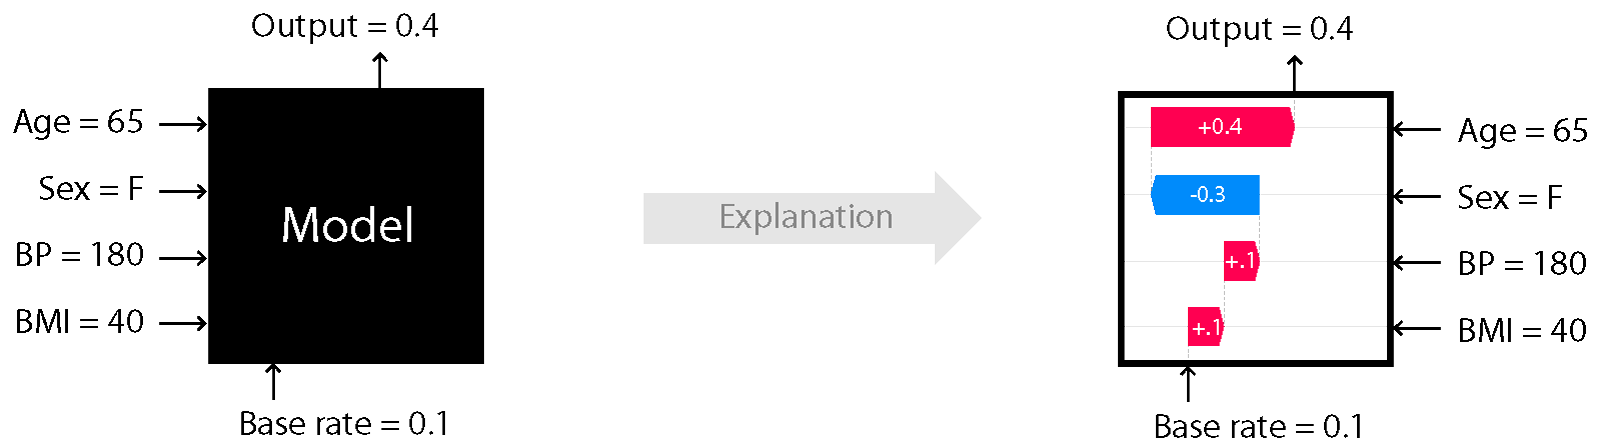
\includegraphics[width=6in]{img/shap_intro.png}
  \caption{SHAP}
  \label{Figure:shap_intro}
\end{figure}
\end{center}

\begin{center}
  \begin{figure}[H]
  \centering
  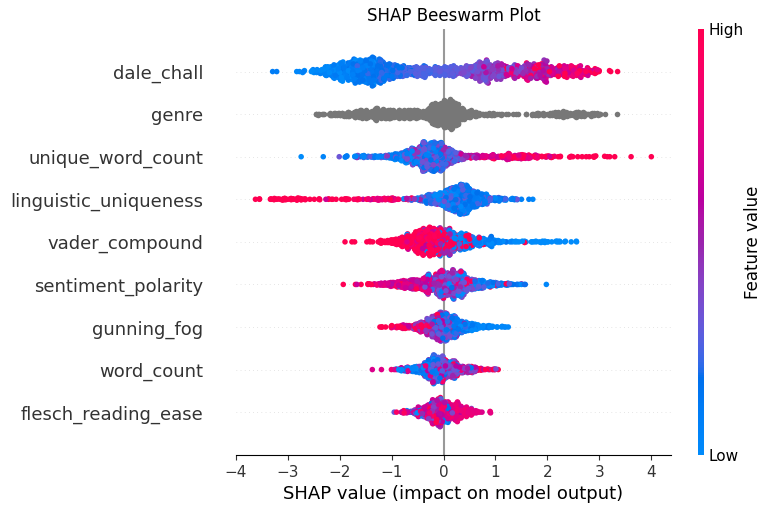
\includegraphics[width=6in]{img/shap_beeswarm.png}
  \caption{Example SHAP beeswarm plot showing impact of some lyrical features
  on the classifier of \textit{explicitness}.}
  \label{Figure:shap_beeswarm}
\end{figure}
\end{center}

\begin{center}
\begin{figure}[H]
  \centering
  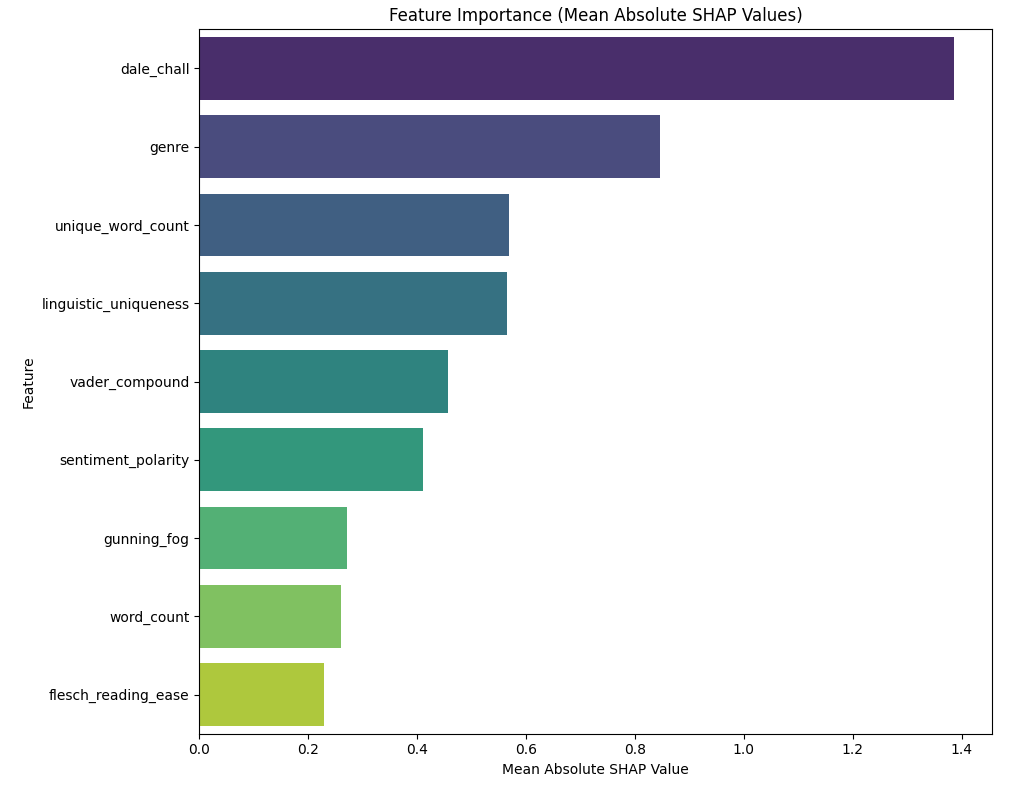
\includegraphics[width=6in]{img/shap_feature_importance.png}
  \caption{Example SHAP feature importance plot showing impact of some lyrical features
  on the classifier of \textit{explicitness}.}
  \label{Figure:shap_feature_importance}
\end{figure}
\end{center}
%---------------------------------------------------------------------------

\subsubsection*{Machine Learning Models}
CatBoost is an algorithm for gradient boosting on decision trees. It's known
for its high predictive accuracy, even without extensive parameter tuning, and
its computational efficiency. In this study it was used to build several
classification and regression models, with the goal of variables like
popularity or explicitness on different subsets of features from the dataset.
The trained models were then subjected to SHAP analysis, uncovering their
decision processes and helping to understand the interactions between the
features and the target variable. Catboost's flexibility, robustness,
compatibility with SHAP and ability to automatically handle categorical
variables and class imbalance.\cite{catboost}


In order to further optimize the performance of the models, the
hyperparameter tuning library \textit{Optuna} was used. Optuna is an
efficient optimization framework that allows to systematically test different
sets of hyperparameter configurations, ensuring the final model achieves
near-optimal performance.\cite{optuna} 

To address the challenges commonly encountered when training ML models on
complex datasets, following techniques were employed:

\begin{itemize}
  \item \textbf{Cross-validation} - cross-validation was used to reduce the
    risk of overfitting and provide a way to reliably calculate model's
    performance metrics. In principle it consists of dividing the training
    data into multiple \textit{folds}, and the model is iteratively trained
    on all folds but one, and evaluated on the one that didn't participate in
    training. In each iteration a different fold is chosen as the evaluation
    fold. This method ensures robust evaluation across the dataset and improved
    model's reliability, at the cost of increased computational time;
  \item \textbf{Class Weights} - due to natural imbalances or skweness in the
    data that was collected, in most classification tasks discussed in this
    paper the target variable (e.g. explicitness) had different number of samples
    representing each value (e.g. there were many more non-explicit songs). That
    kind of imbalance would lead to model favouring the majority class, and
    therefore performing poorly. Catboost offers a built-in mechanism to handle
    class imbalance by assigning different penalties for misclassifications
    of specific classes, improving model's performance across all classes;
  \item \textbf{Out of sample evaluation} - model's performance was evaluated
    on data that was completely excluded from the training process, ensuring
    reliable measurement of model's ability to generalize on unseen data.
\end{itemize}

\section{Dimensionality Reduction - Principal Component Analysis (PCA)}
\label{sec:dimensionalityreduction}
Principal Component Analysis (PCA) is a dimensionality reduction technique
that reduces the number of features by transforming them into \textit{principal
components} that retain most of the original information. It works by
converting potentially correlated variables in to smaller sets of less correlated
variables, in a way that preserves as much of the variance from the original
data as possible. It's often applied on large datasets to reduce dimensionality
and improve generalization and performance by reducing noise and redundancy
in the data. Fig.~\ref{Figure:pca} illustrates how PCA works. \cite{pca} 

In this study it was applied to the TF-IDF and Word2Vec vectors extracted from
the song lyrics. The vectors in their original form were problematic due  to
increased computational complexity and risk of overfitting the trained models.

The application of PCA reduced their dimensionality while preserving as much
useful information as possible, improving the computational efficiency and 
the interpretability of the data, which is particularly important in context of
XAI.

\begin{center}
\begin{figure}[H]
  \centering
  \includegraphics[width=6in]{img/pca.png}
  \caption{A scatterplot showing the relationship between PC1 and PC2 when PCA
  is applied to a dataset. PC1 and PC2 axis are perpendicular to each other.\cite{pca}}
  \label{Figure:pca}
\end{figure}
\end{center}


\section{Topic Modelling - Latent Dirichlet Allocation (LDA)}
\label{sec:topicmodelling}

Latent Dirichlet allocation is an unsupervised machine learning algorithm used
for topic modeling to uncovering the central topics and their distributions
across the dataset.\cite{lda}

In this study LDA was applied on the lyrics to identify commonly occuring
topics in songs. The algorithm automatically found the best number of topics
and they were visualized using \textit{pyldavis}\cite{pylda} library. For each
topic its most representative words were extracted that in combination with
other features allowed to better characterize them and understand frequently
occuring themes in the lyrics.



\section{Statistical Methods}
\label{sec:statisticalmethods}

Statistical methods provided a foundation for descriptive data analysis, mainly
exploration of relationships between variables and identification of distinctive
genre traits, as well as hypothesis validation.

\subsection{Pearson Correlation}

It measures linear relationship between two continuous variables. The resulting
coefficient is a value between -1 to 1 and is computed as follows: 

\[
r = \frac{\sum{(x_i - \bar{x})(y_i - \bar{y})}}{\sqrt{\sum{(x_i - \bar{x})^2} \sum{(y_i - \bar{y})^2}}}
\]

\noindent \noindent where:
\begin{itemize}
    \item \( x_i \) and \( y_i \): The data points of the two variables;
    \item \( \bar{x} \) and \( \bar{y} \): The mean values of the variables.
\end{itemize}

\noindent \noindent Interpretation:
\begin{itemize}
  \item An \textit{r} value close to 1 indicates very strong positive linear
    relationship;
  \item An \textit{r} value close to -1 suggests very strong negative linear
    relationship;
  \item An \textit{r} value close to 0 means there is little to no relationship.
\end{itemize}



\subsection{Bootstrap Testing}

Bootstrap testing was used to verify hypotheses specified in the research
objectives. It's a resampling-based statistical technique that estimates the
variability of a statistic (e.g. mean or median)  by repeatedly sampling its
values from the dataset with replacement. It's highly versatile since it
doesn't rely on strong distributional assumptions. Fig.~\ref{Figure:bootstrap}
shows an example result of a bootstrap test.


\begin{center}
\begin{figure}[H]
  \centering
  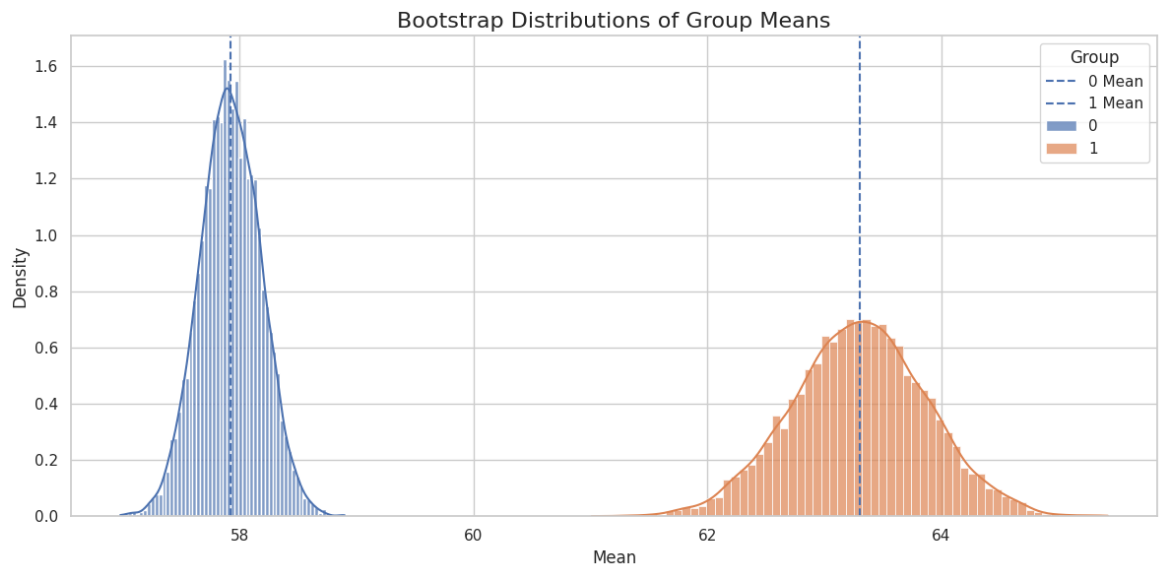
\includegraphics[width=6in]{img/bootstrap.jpg}
  \caption{Illustration of bootstrap resampling: The distribution of the
  statistic (e.g., mean) of the target variable for two different samples
(called groups). This demonstrates the variability of the statistic across
resampled datasets.}
  \label{Figure:bootstrap}
\end{figure}
\end{center}

\subsection{Analysis of Variance - ANOVA}
ANOVA is a statistical method used to compare the means of three or more groups
to determine if there is a statistically significant difference between them.
It tests the hypothesis that the means of all groups are equal against the
alternative hypothesis that at least one group mean is different.

\subsubsection*{Hypotheses}
\begin{itemize}
  \item \textbf{Null Hypothesis ($H_0$)}: All group means are equal;
  \item \textbf{Alternative Hypothesis ($H_a$)}: At least one group mean is
    different.
\end{itemize}

\noindent \noindent To verify the hypotheses two types of variation have to
be calculated:

\subsubsection*{Between-Group Variation}

This variation measures the differences between the means of groups. It
captures how much the group means differ from the overall mean.
\[
\text{Between-group \  variation} = \sum_{i=1}^{k} n_i (\bar{x}_i - \bar{x})^2
\]

\noindent \noindent where:
\begin{itemize}
    \item \(n_i\): Number of samples in group \(i\);
    \item \(\bar{x}_i\): Mean of group \(i\);
    \item \(\bar{x}\): Overall mean.
\end{itemize}


\subsubsection*{Within-Group Variation}
It measures the variability of data points within each group.

\[
\text{Within-group  \ variation} = \sum_{i=1}^{k} \sum_{j=1}^{n_i} (x_{ij} - \bar{x}_i)^2
\]

\noindent \noindent where:
\begin{itemize}
    \item \(x_{ij}\): Individual data point in group \(i\);
    \item \(\bar{x}_i\): Mean of group \(i\).
\end{itemize}



\subsubsection*{F-Statistic Calculation}
In order to calculate the \textbf{F-statistic} and verify the hypotheses
the MSB and MSW have to be calculated:

\begin{itemize}
    \item \textbf{Mean Square Between (MSB)}:
    
    Formula:
    \[
    \text{MSB} = \frac{\text{Between-group variation}}{\text{df}_{\text{between}}}
    \]
    \noindent \noindent where:
    \begin{itemize}
        \item \( \text{df}_{\text{between}} = k - 1 \): Degrees of freedom (in
          that case number of groups minus one).
    \end{itemize}
\end{itemize}

\begin{itemize}
    \item \textbf{Mean Square Within (MSW)}:
    
    Formula:
    \[
    \text{MSW} = \frac{\text{Within-group \ variation}}{\text{df}_{\text{within}}}
    \]
    \noindent \noindent where:
    \begin{itemize}
        \item \( \text{df}_{\text{within}} = N - k \): Total number of observations minus the number of groups.
    \end{itemize}
\end{itemize}


\noindent \noindent The \textbf{F-statistic} is calculated as the ratio of
between-group variance to within-group variance:
\[
F = \frac{\text{MSB}}{\text{MSW}}
\]


Based on the calculated F-statistic, p-value can be calculated and depending on
the value and the chosen significance level the null hypothesis $H_0$ will be
rejected or not.
